% !TEX root = ../Thesis.tex
\chapter{Evaluation Results}
\label{app:evaluation-results}

\begingroup
\selectlanguage{english}
\setlength{\emergencystretch}{3em}

This appendix presents the complete results of the feedback. The full wording of each question is not repeated here. The complete questions, answer options, and structure of the questionnaire can be found in Appendix~\ref{app:evaluation-questionnaire}.

The horizontal scale from 0 to 100\,\% shows how the responses are distributed. The width of each coloured segment shows the percentage of responses in that category, while the number inside the segment shows the number of responses. $n$ is the number of participants who answered the question.

\section{Sample and Device Use}

\begin{figure}[H]
  \centering
  \subbottom[Affinity for technology  ($n=9$)]{
    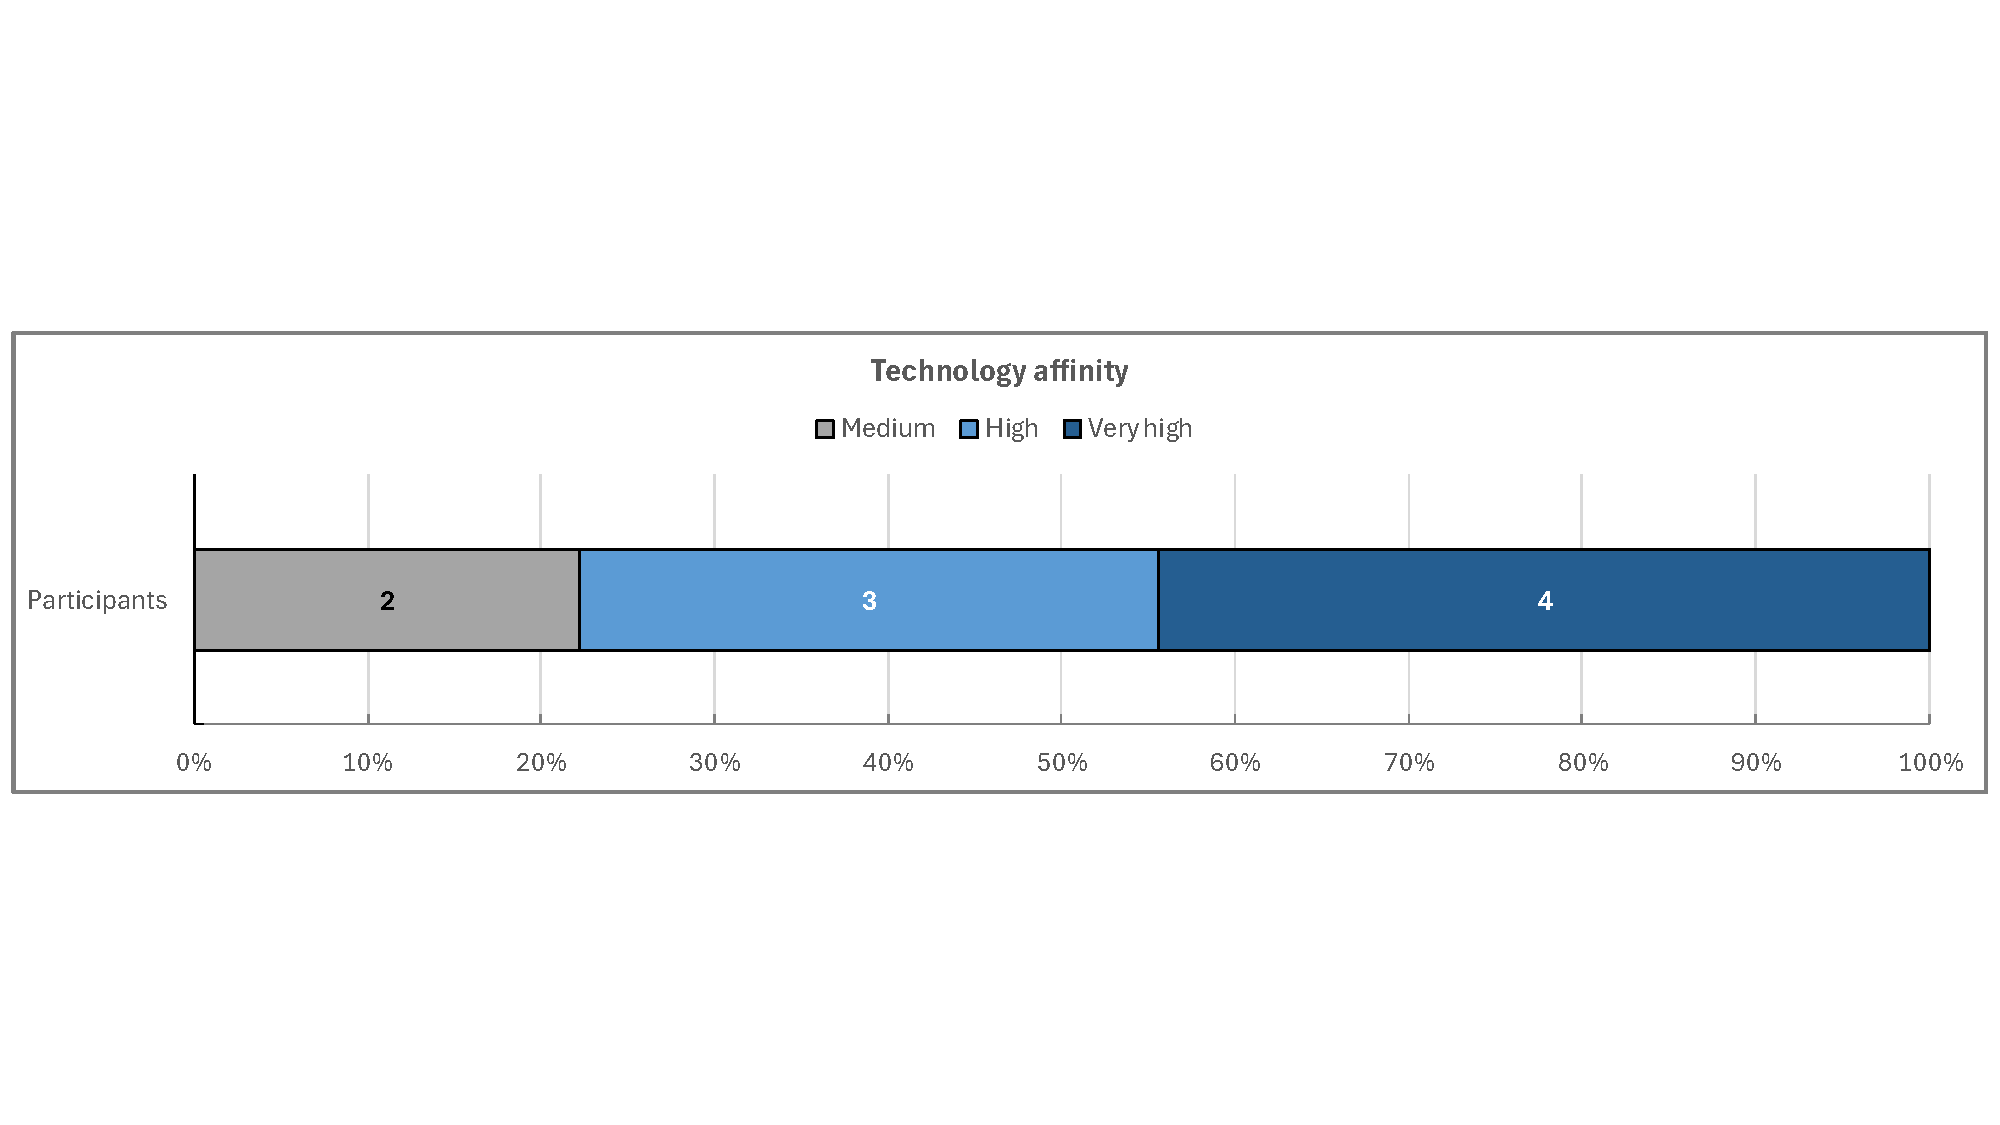
\includegraphics[width=0.96\textwidth]{Figures/app-c-01-technology-affinity.pdf}
    \label{fig:appendix-technology-affinity}
  }
  \medskip

  \subbottom[VR experience ($n=9$)]{
    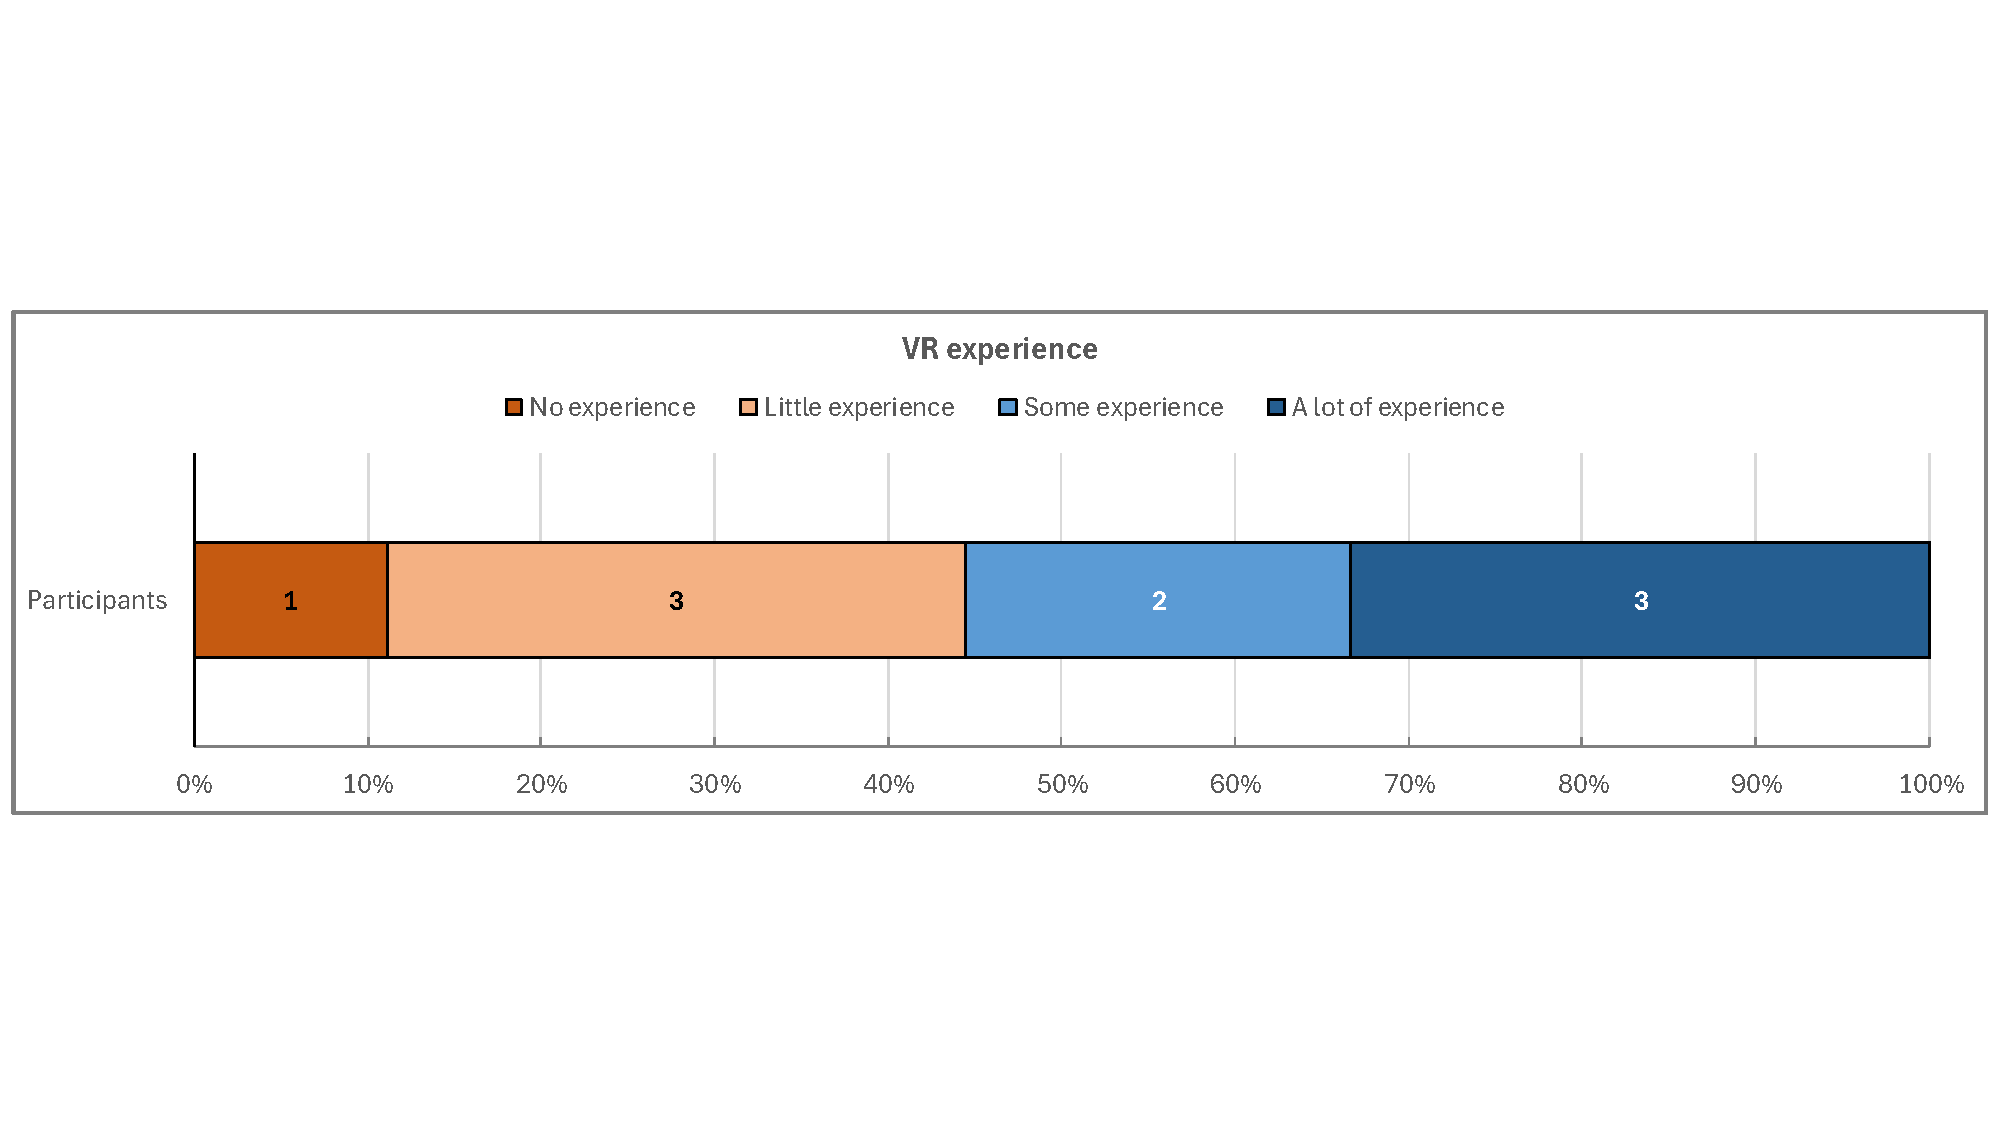
\includegraphics[width=0.96\textwidth]{Figures/app-c-02-vr-experience.pdf}
    \label{fig:appendix-vr-experience}
  }
  \caption[Technology affinity and VR experience]{Distribution of affinity for technology and previous VR experience in the sample.}
  \label{fig:appendix-sample-characteristics}
\end{figure}

\begin{figure}[H]
  \centering
  \subbottom[Previously used VR headsets ($n=9$, multiple answers possible)]{
    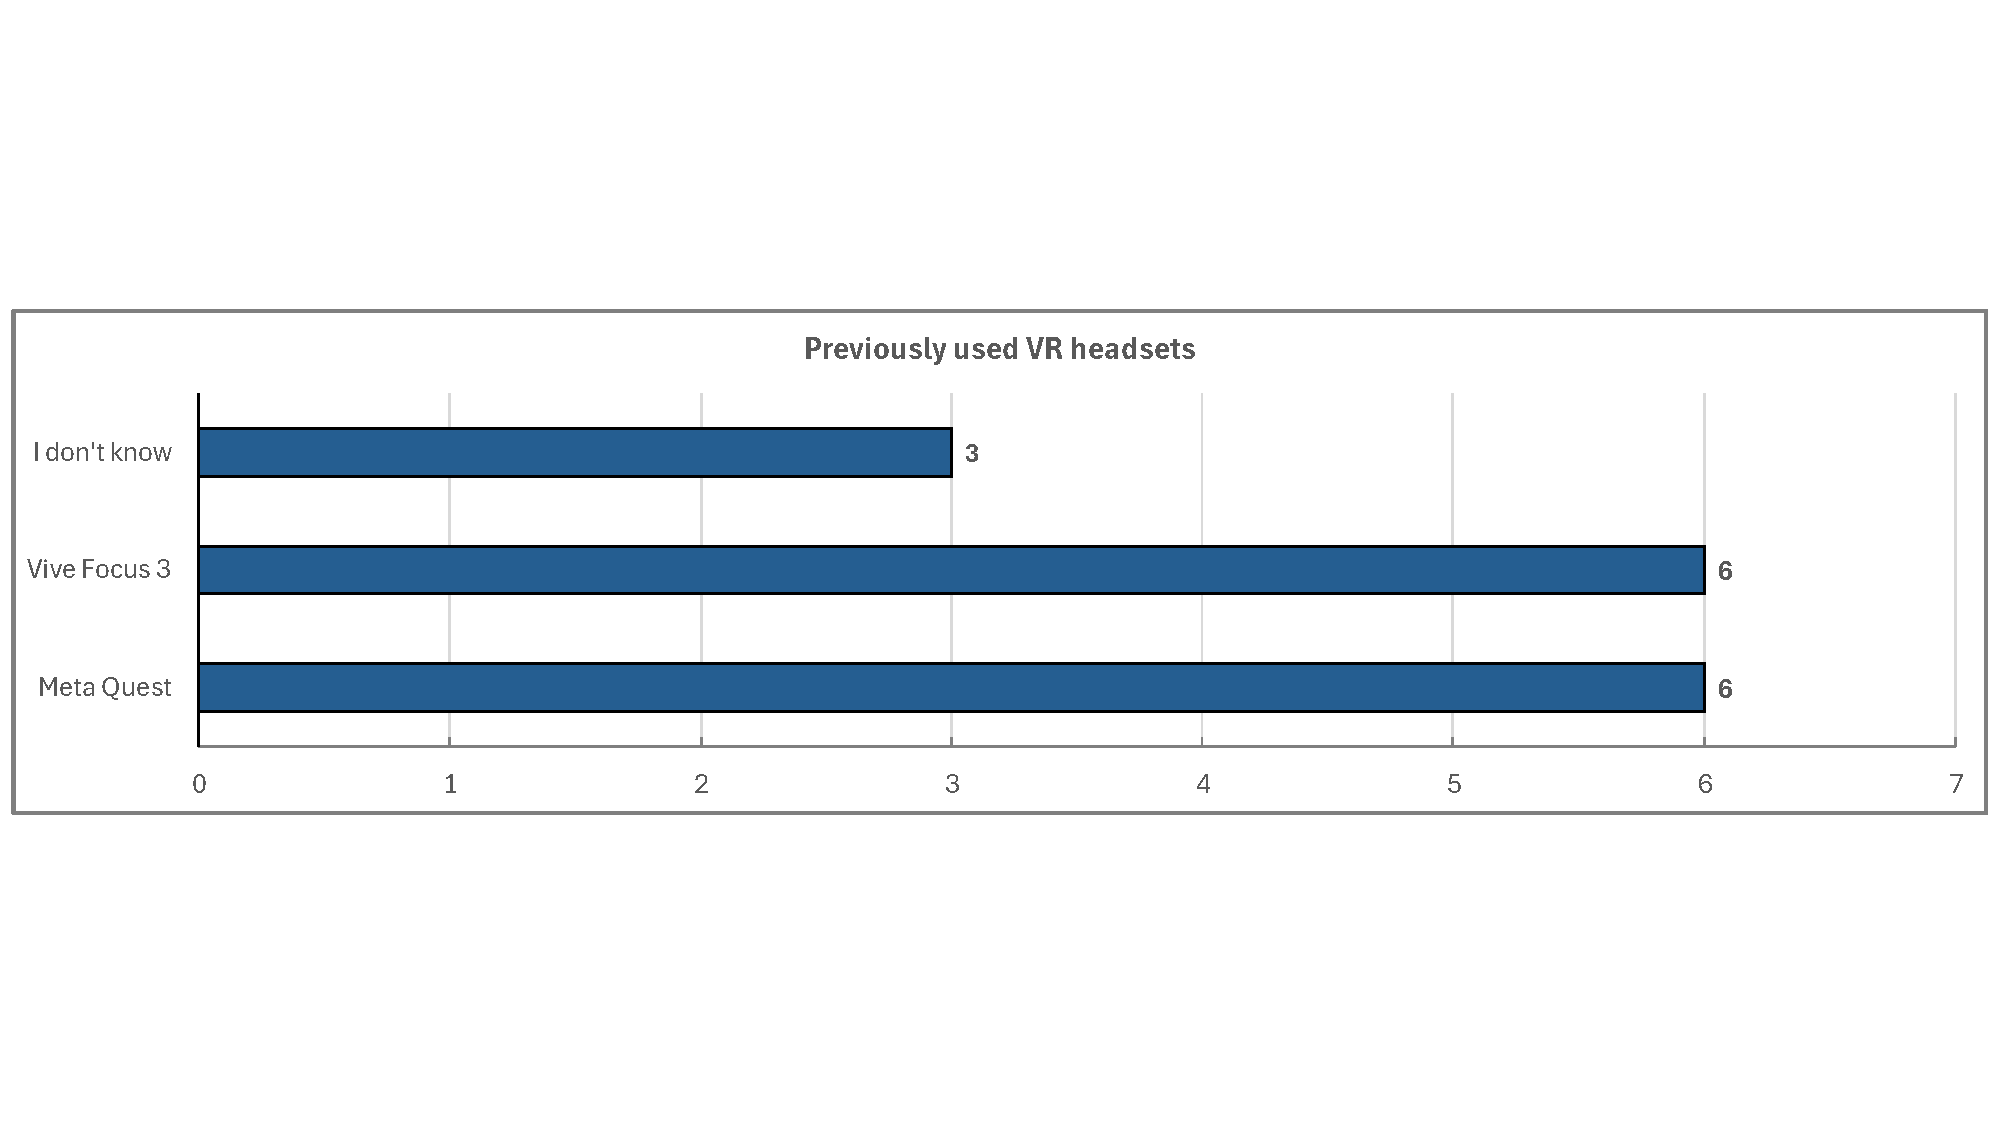
\includegraphics[width=0.9\textwidth]{Figures/app-c-03-previously-used-headsets.pdf}
    \label{fig:appendix-previous-headsets}
  }
  \medskip

  \subbottom[Tested versions ($n=9$)]{
    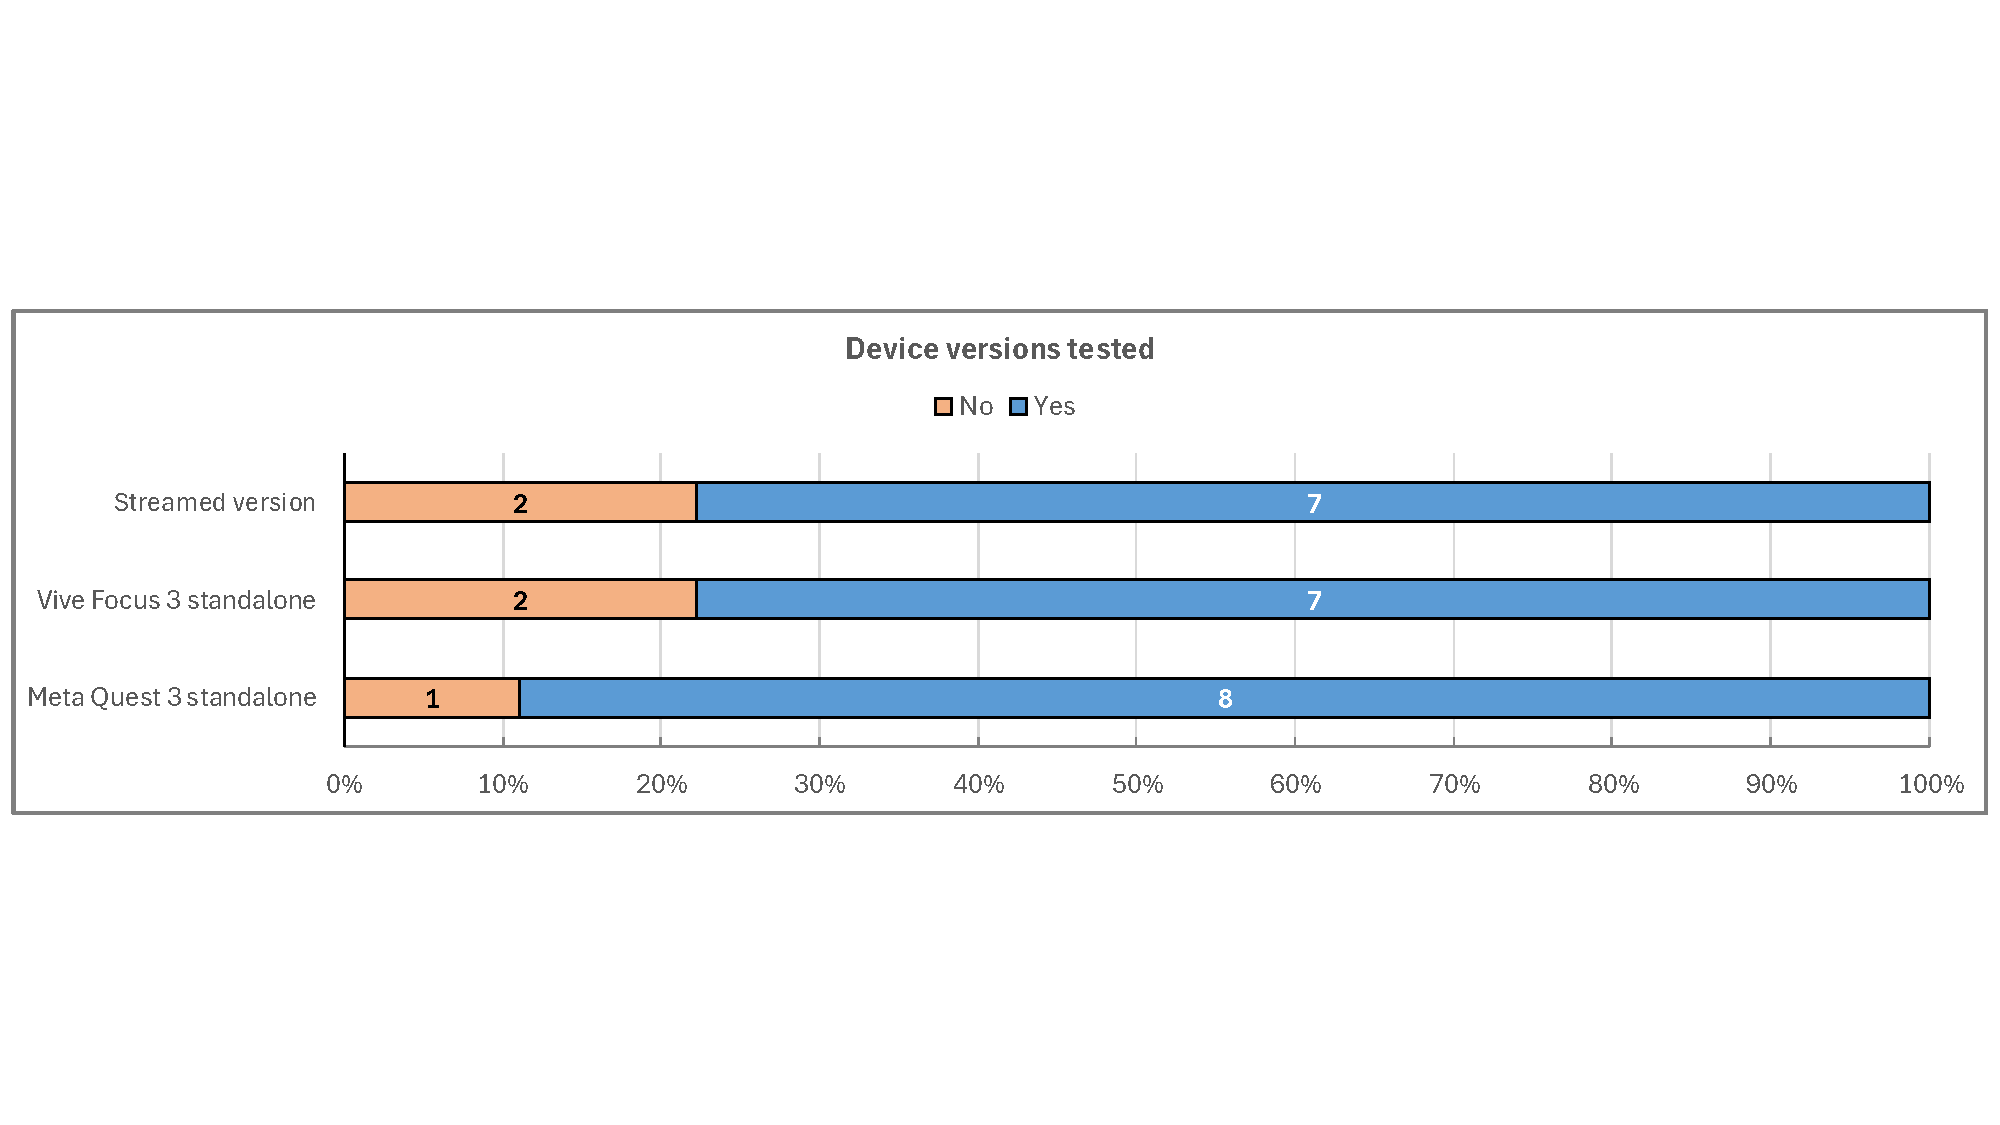
\includegraphics[width=0.9\textwidth]{Figures/app-c-04-tested-device-versions.pdf}
    \label{fig:appendix-tested-versions}
  }
  \caption[Device use and tested versions]{Previously used devices and participation in the individual test phases. In (a), the horizontal axis shows the number of responses. In (b), it shows the percentage of participants.}
  \label{fig:appendix-device-use}
\end{figure}

\section{System Usability Scale}

\begin{table}[H]
\begin{tabular}{@{}lrrrrrrrrr@{}}
\toprule
Person & P1 & P2 & P3 & P4 & P5 & P6 & P7 & P8 & P9 \\
\midrule
SUS & 82.5 & 77.5 & 82.5 & 75.0 & 70.0 & 77.5 & 82.5 & 80.0 & 82.5 \\
\bottomrule
\end{tabular}
\caption{Individual SUS scores.}
\end{table}

\begin{figure}[H]
  \centering
  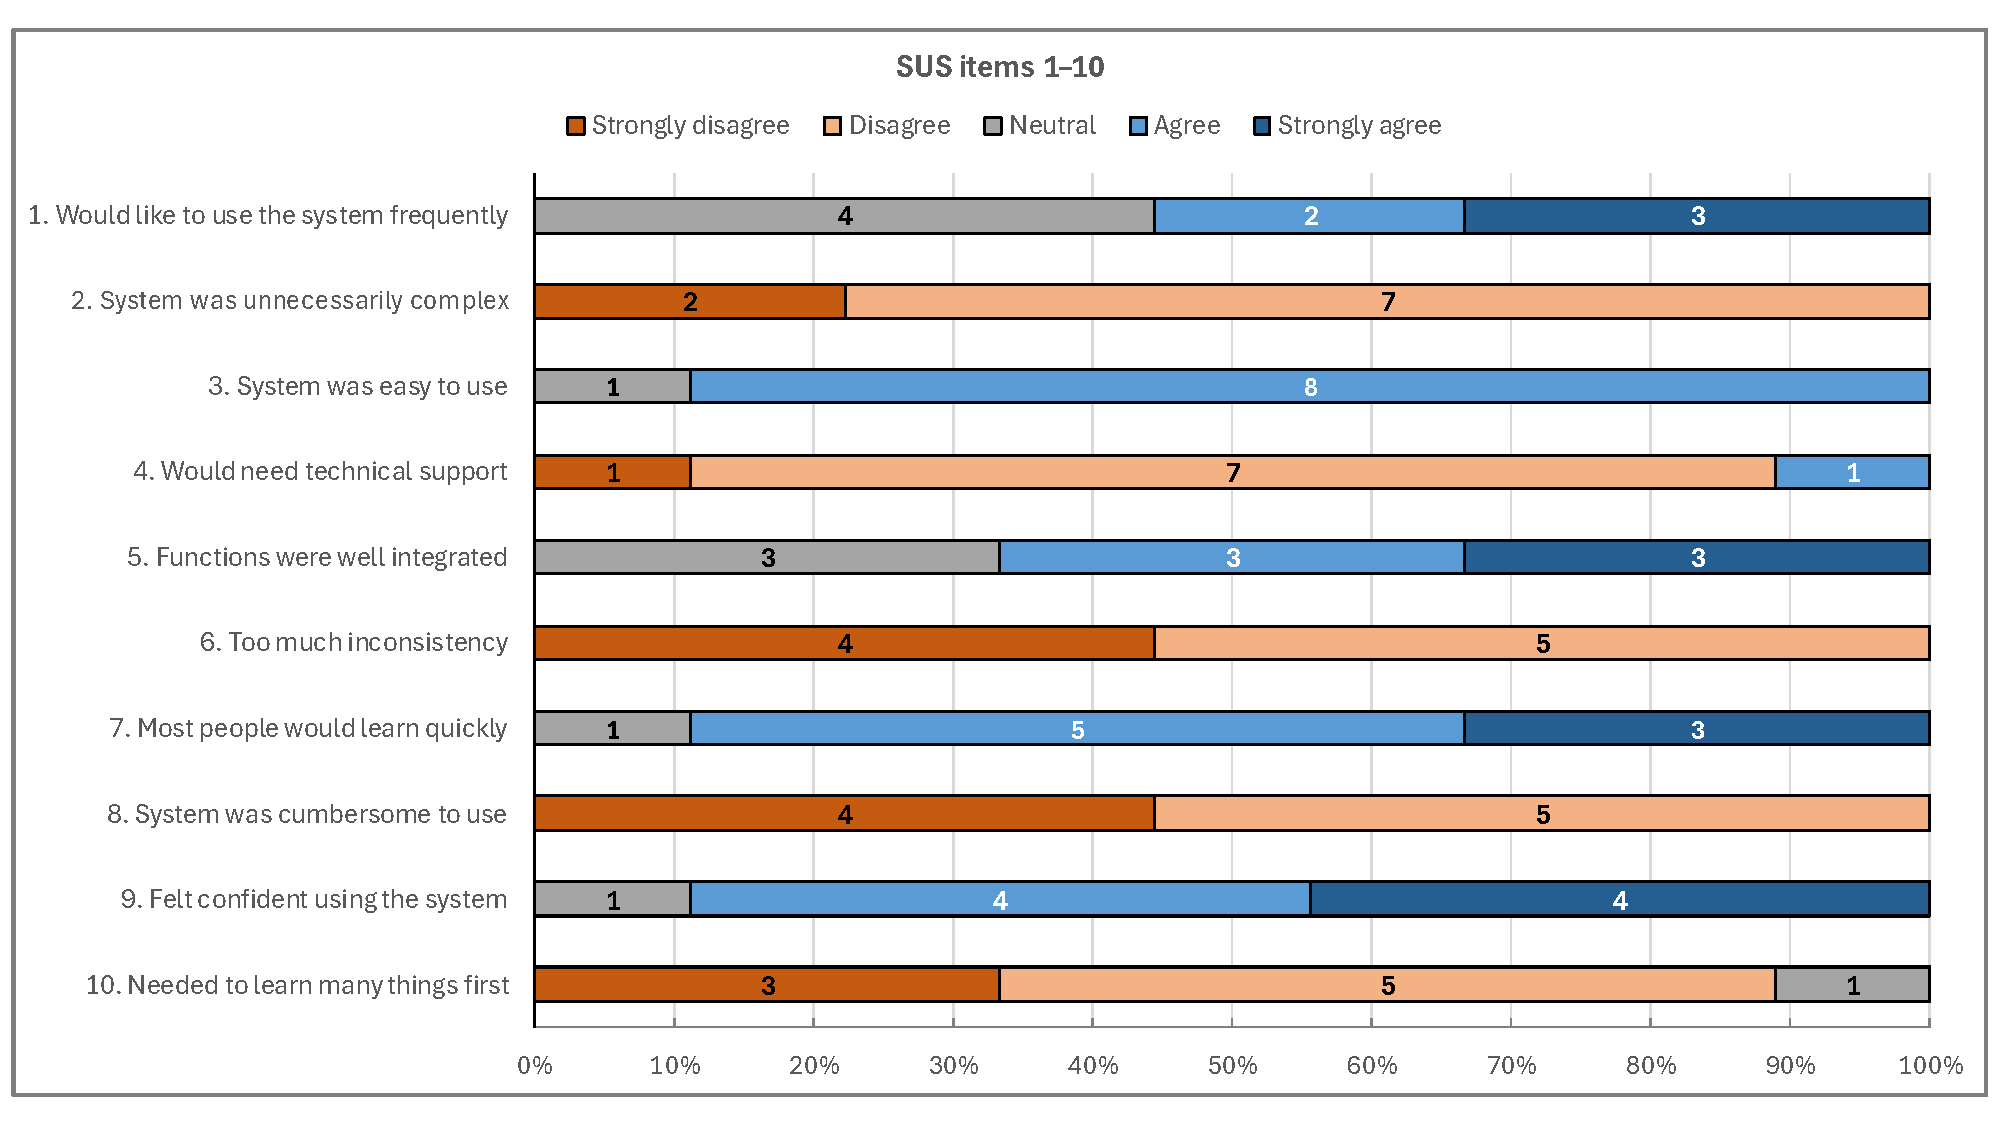
\includegraphics[width=0.88\textwidth]{Figures/app-c-05-sus-item-responses.pdf}
  \caption[Distributions of the SUS items]{Responses to the ten SUS items ($n=9$).}
  \label{fig:appendix-sus-items}
\end{figure}

\section{Device-Specific Ratings}

\begin{figure}[H]
  \centering
  \subbottom[Quest Standalone ($n=8$)]{
    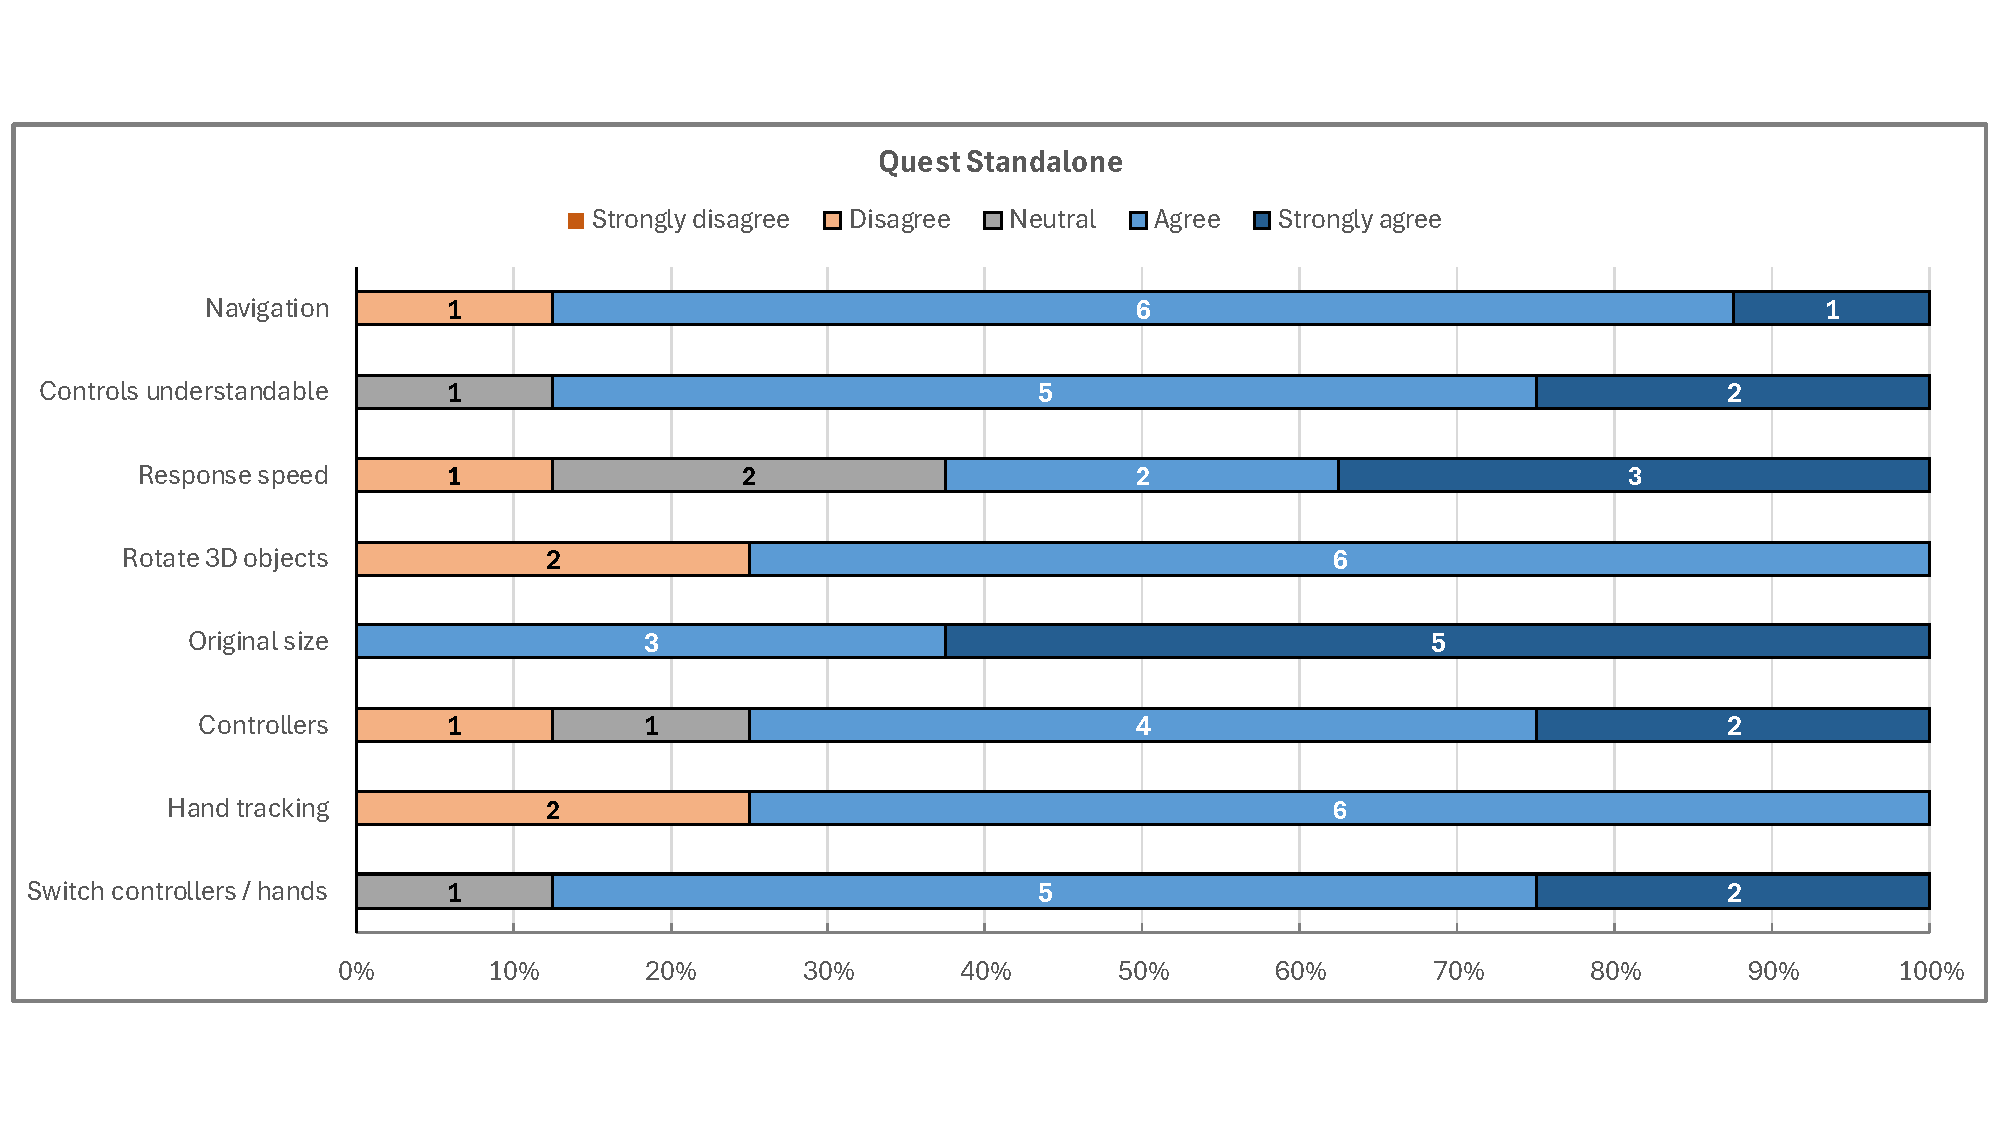
\includegraphics[width=0.88\textwidth]{Figures/app-c-06-quest-standalone-responses.pdf}
    \label{fig:appendix-quest-standalone}
  }
  \smallskip

  \subbottom[Focus Standalone ($n=7$)]{
    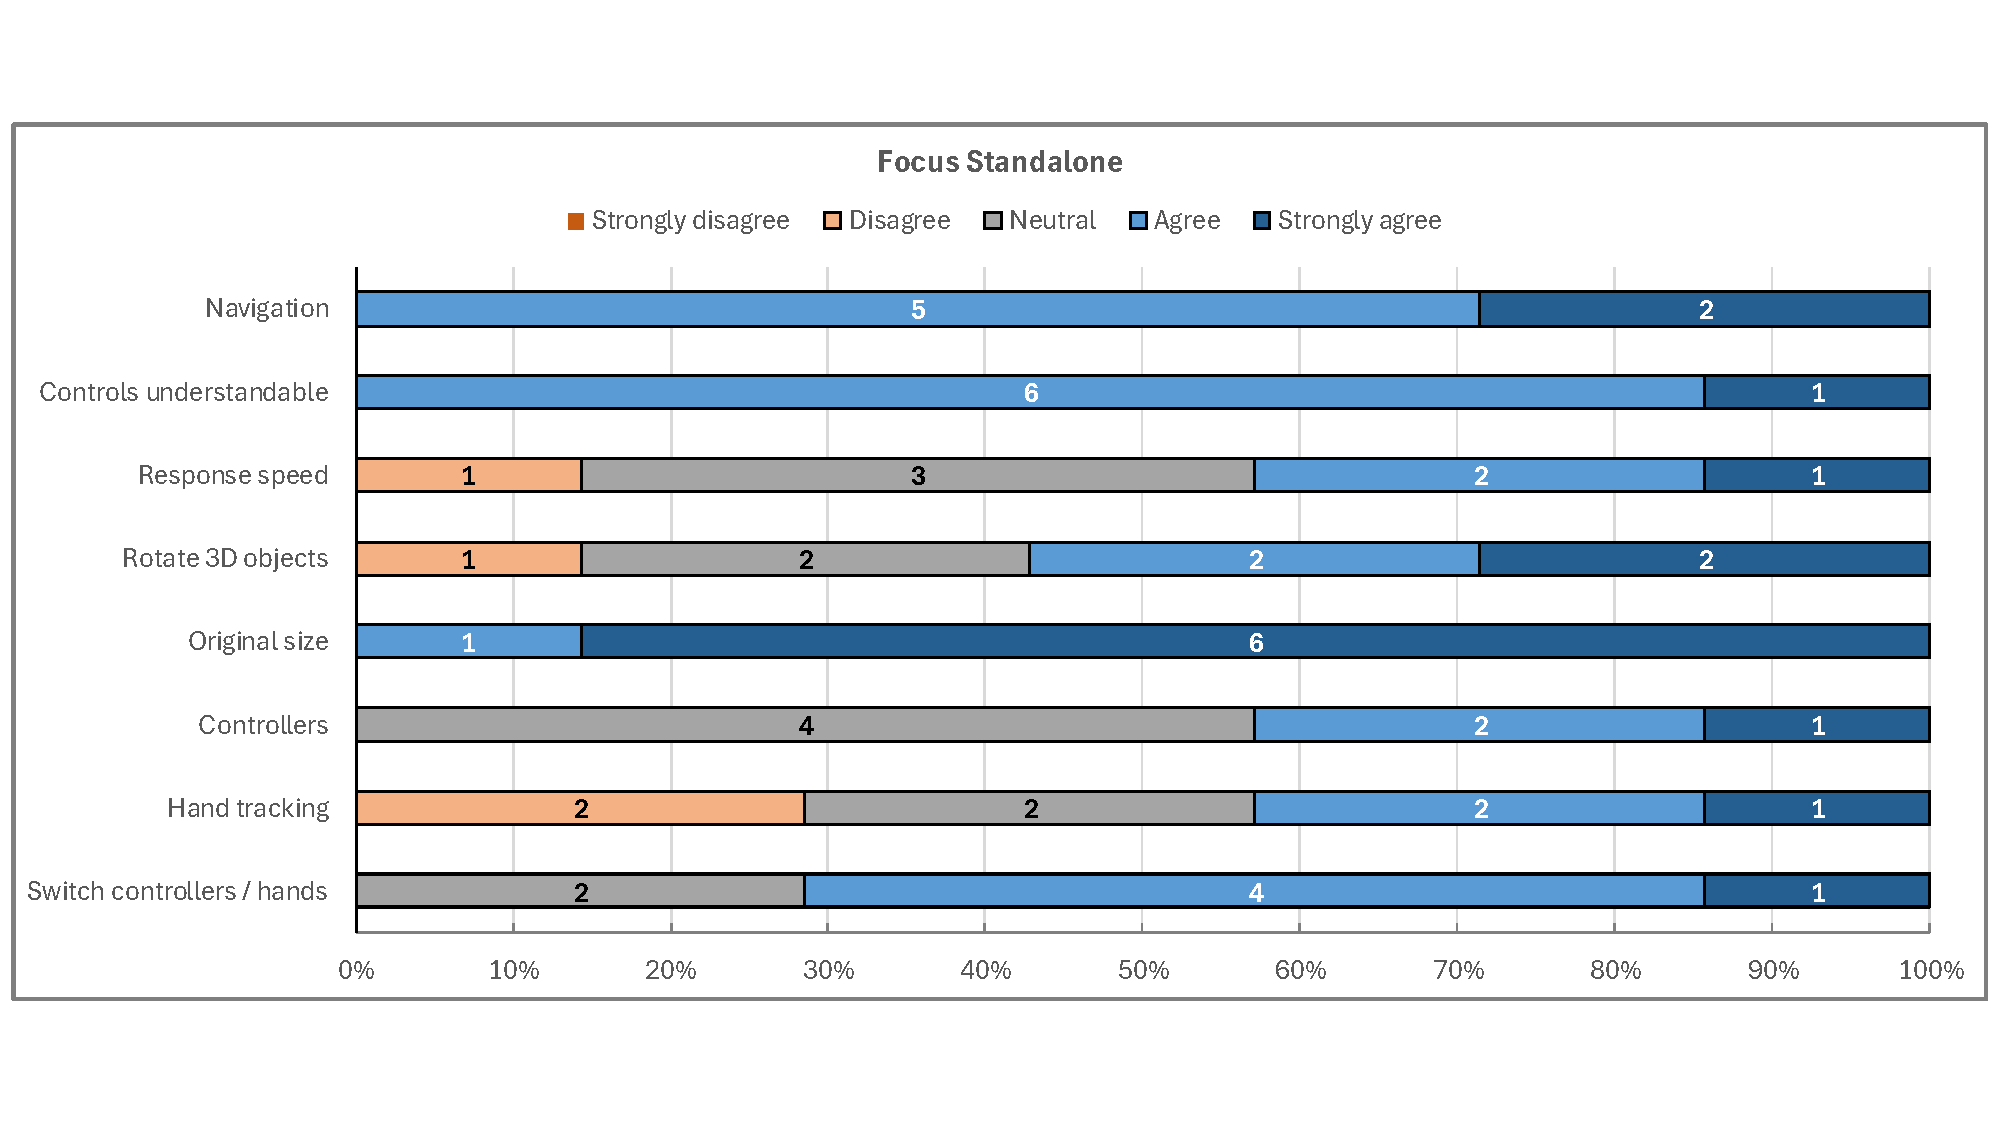
\includegraphics[width=0.88\textwidth]{Figures/app-c-07-focus-standalone-responses.pdf}
    \label{fig:appendix-focus-standalone}
  }
  \smallskip

  \subbottom[Quest Streaming ($n=7$)]{
    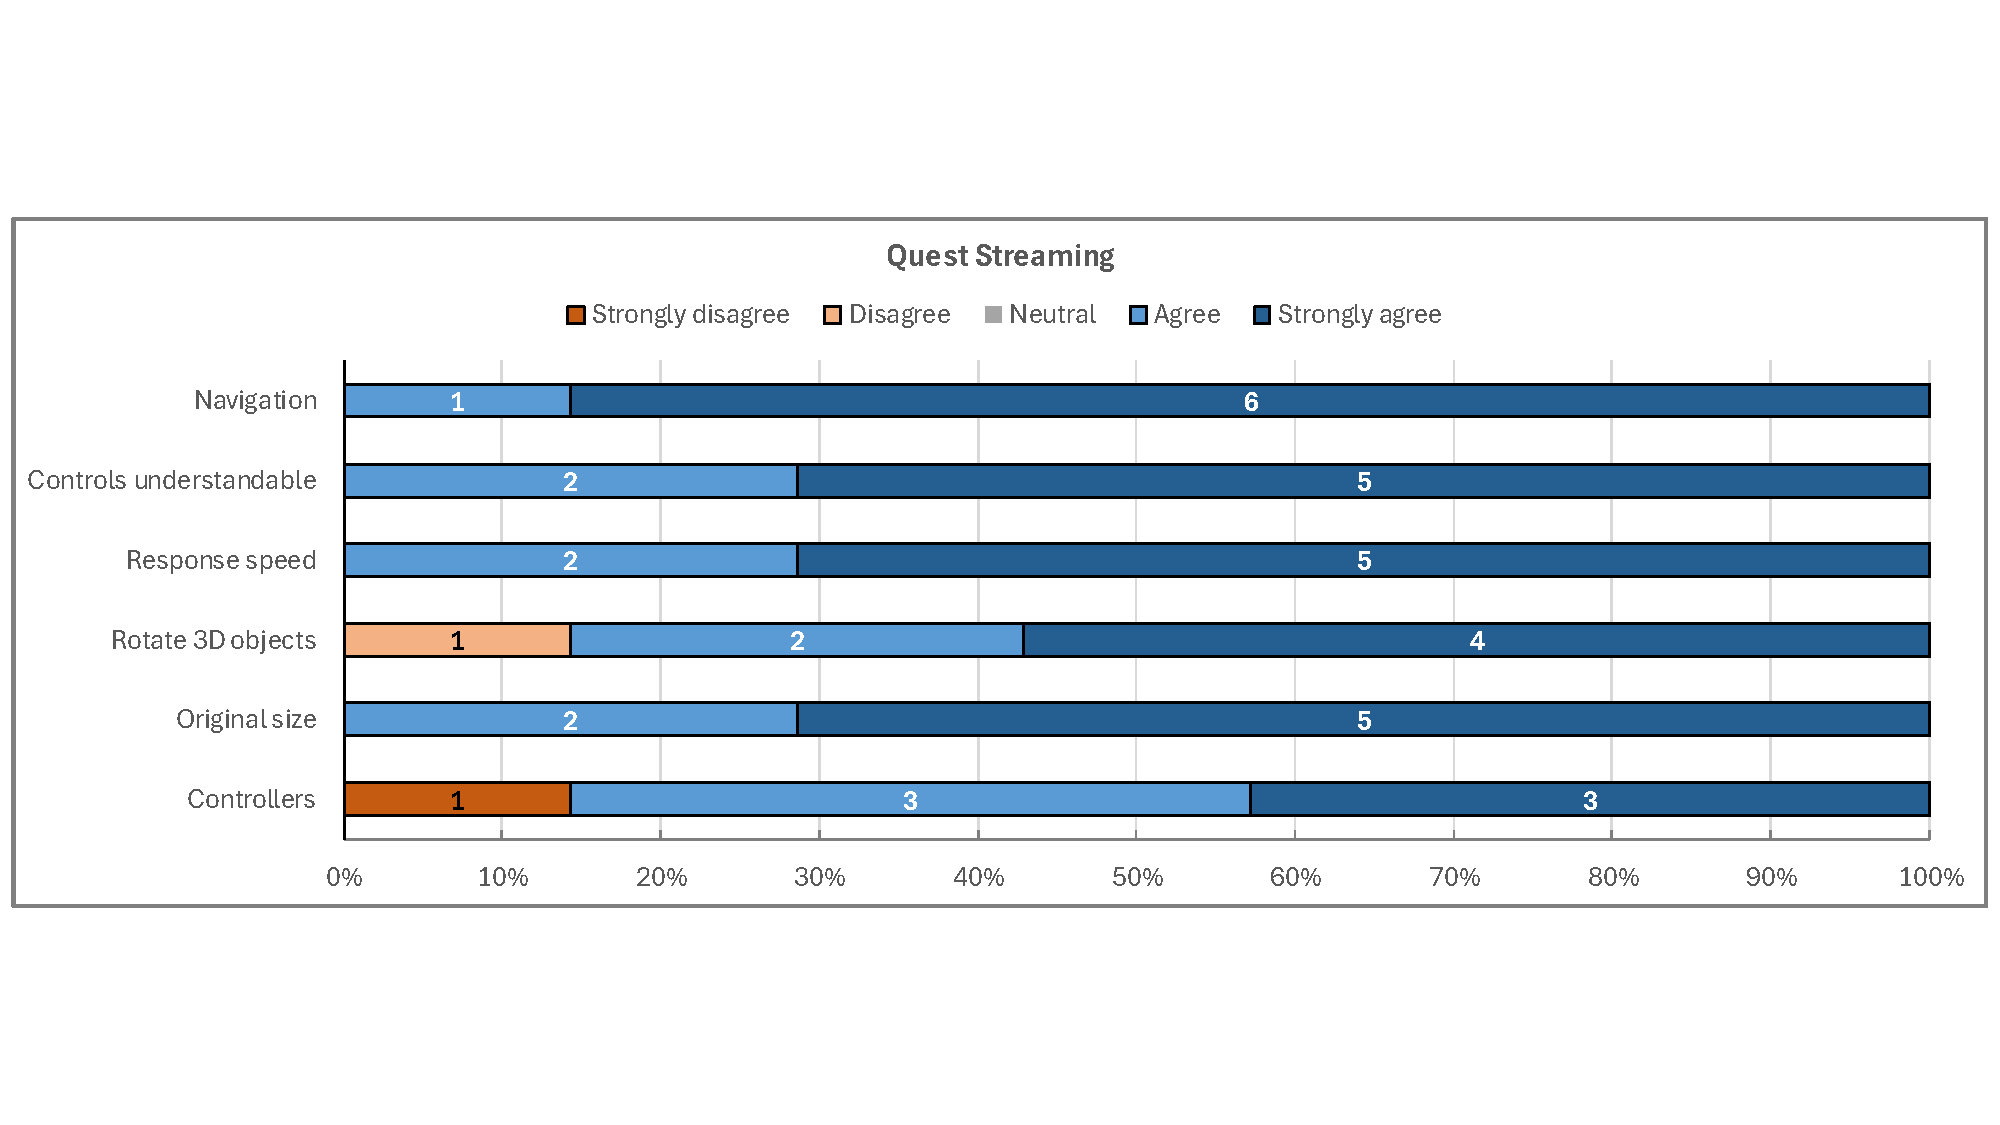
\includegraphics[width=0.88\textwidth]{Figures/app-c-08-quest-streaming-responses.pdf}
    \label{fig:appendix-quest-streaming}
  }
  \caption[Device-specific response distributions]{Response distributions for the three tested versions.}
  \label{fig:appendix-device-responses}
\end{figure}

\section{Design and Visual Appearance}
\begin{figure}[H]
  \centering
  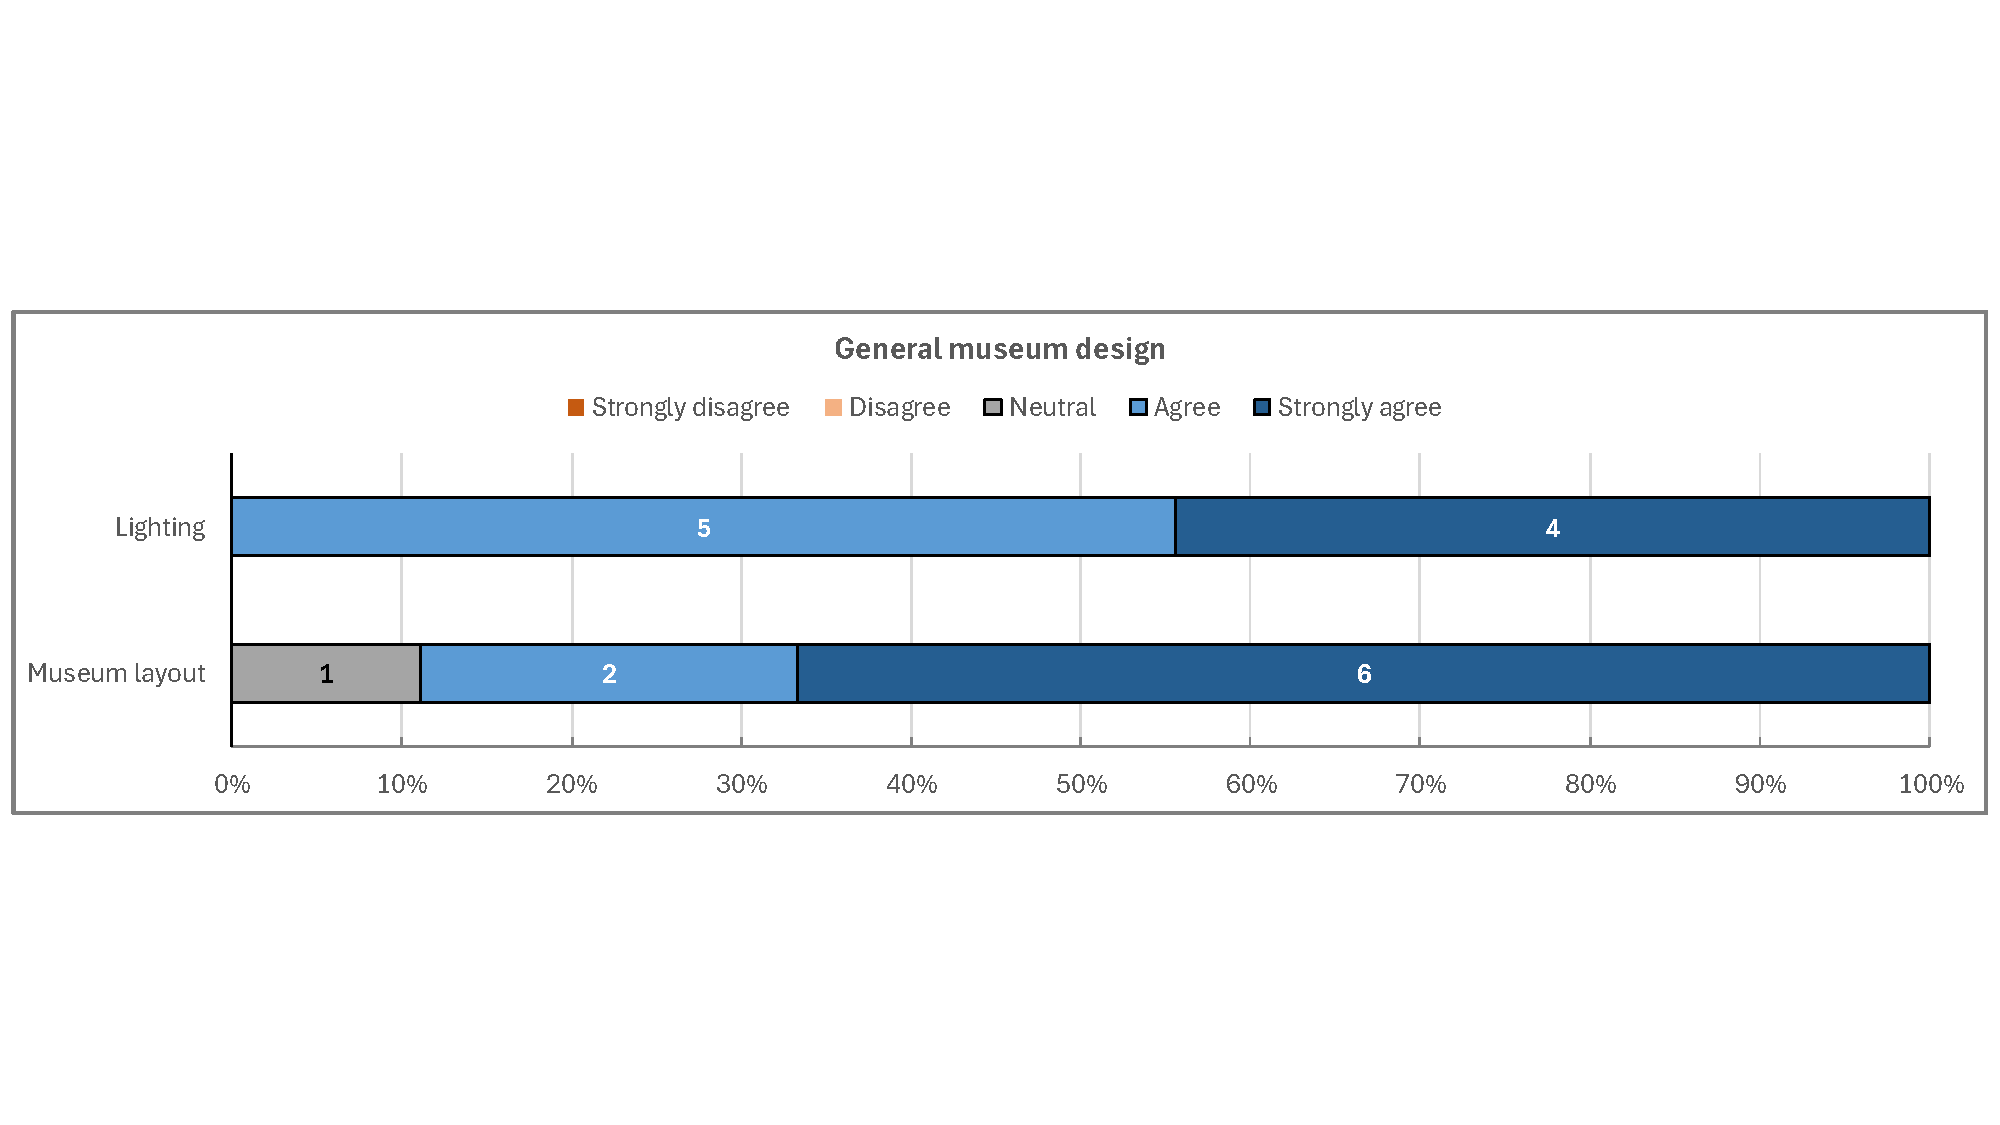
\includegraphics[width=\textwidth]{Figures/app-c-09-general-museum-design.pdf}
  \caption[Ratings of the general museum design]{Responses for the general museum design ($n=9$).}
  \label{fig:appendix-general-design}
\end{figure}

\section{Qualitative Feedback}

The following six responses were given by the participants exactly as written:

\begin{itemize}[leftmargin=*]
  \item See Tutorial again, interactive tutorial, information about exhibits

  Overall very well done!
  \item Loading bar slighly lower not so far up. Re-Display the interaction directions if the user is idle for longer periods. Highlighting grabbed trigger more as soon as it is active.
  \item A clearer feedback signal on semantic search updating the museum exponents, like a brief change of lighting or some kind of outward wave, something that clearly signals that the entire room is being affected.
  \item Showing metadata. Textual input is a bit cumbersome, probably input method could be improved. Option to force 3d results. Collision improvments.
  \item More options to interact with the objects, option to go back and forth between searches.
  \item Per default: lower movement and rotation speed
\end{itemize}

Besides the written feedback, participants also made three suggestions verbally:

\begin{itemize}[leftmargin=*]
  \item Make the tutorial available while the application is running.
  \item Show button labels when users look at the virtual controllers/hands.
  \item Allow selecting the interaction sphere to rotate the 3D model with the joystick.
\end{itemize}

\selectlanguage{english}
\endgroup
